\documentclass[custom, plainsections]{sciposter}

%%%%%%%%%%%%%%%%%%%%%%%%%%%%%%%%%%%%%%%%%%%%%%%%%%%%%%%%%%%%%%%%%%%%%%
% Modify paper size and font size in papercustom.cfg in your tex install
% e.g. something like:
%  /usr/local/texlive/2010/texmf-dist/tex/latex/sciposter/papercustom.cfg
%  /usr/share/texmf-texlive/tex/latex/sciposter/papercustom.cfg
%
%\renewcommand{\papertype}{custom}
%\renewcommand{\fontpointsize}{14pt}
%\setlength{\paperwidth}{31.7cm}
%\setlength{\paperheight}{45.7cm}
%\renewcommand{\setpspagesize}{
%  \ifthenelse{\equal{\orientation}{portrait}}{
%    \special{papersize=31.7cm,45.7cm}
%    }{\special{papersize=45.7cm,31.7cm}
%    }
%  }
%%%%%%%%%%%%%%%%%%%%%%%%%%%%%%%%%%%%%%%%%%%%%%%%%%%%%%%%%%%%%%%%%%%%%%

\usepackage[ascii]{inputenc}
\usepackage[greek, english]{babel}
\usepackage[pdftex]{graphicx}
\usepackage{fancyvrb}
\usepackage{color}
\usepackage{cwpuzzle}
\usepackage{multicol}

\setlength\columnseprule{0.2pt}

<< pygments['pastie.tex'] >>

\renewcommand{\rmdefault}{ptm}
\newcommand{\megasize}{\fontsize{100pt}{20pt}\selectfont}

\setmargins[1.5cm]

\pagenumbering{arabic}

\title{Dexy News}
\author{Ana Nelson}
\begin{document}
\rmfamily

\begin{megasize}

\includegraphics{../logo.pdf}
\hspace{0.7in}
Dexy News
\end{megasize} \hfill February 2012


\begin{multicols*}{3}

\small
<< d['001.c|pyg|l'] >>

\vspace{0.5cm}

\PARstart{D}{exy} is a new open source software project for building and automating documents. Dexy will help you present your code, data and graphs elegantly, easily and correctly in any format, even a blog. This newspaper was created using Dexy, and in it we discuss how Dexy was designed and what it can do.

\vspace{10pt}
\hrule
\vspace{10pt}

\large
Dexy for Code
\small

\vspace{5pt}

\PARstart{I}{f} you write code, even just the occasional R or Matlab script, then you also need to write about code, and Dexy can help. Dexy makes it easy to do things like keep a personal code journal, write blog posts including code samples, and incorporate code into journal articles, books or any other documents you need to write. For example, you can include syntax highlighted code like this (it's much prettier in colour but this newspaper is black and white):

<< d['001.c|pyg|l'] >>

\noindent and you can see the results of running this code, like this:

\begin{Verbatim}
<< d['001.c|c'] >>
\end{Verbatim}

Dexy easily supports multiple languages in a single document, for example here is some R:

<< d['hello.R|r|pyg|l'] >>

With Dexy, you never type dead code into your document, instead Dexy reads your source code and transforms it according to filters that you specify. These filters do things like run your code through an interpreter, apply syntax highlighting, or both. Filters can do just about anything, and you can chain filters together.


This approach makes it fast and natural to write documents which incorporate code. You write code in code files using your text editor or IDE of choice, and write text in your document in any* format you want, then use Dexy to bring them together. This way your code is testable, runnable and can be included in many different documents (such as your paper, your poster and your presentation slides).

*In theory, Dexy should be able to work with any text-based format (such as plain text, \LaTeX, or HTML), any binary format which can be produced from a text-based markup, or any binary format which can be accessed via a scriptable interface. If you don't see your preferred format, then please ask us via the forum http://discuss.dexy.it or twitter @dexyit and we'll do our best to support it. Obviously, it's easier to support open source formats since we can install these and test them out, but we'll do our best to help with proprietary formats.

\vspace{30pt}

\large
Dexy for Science
\vspace{5pt}
\small

\PARstart{D}{exy} was designed to be a powerful tool for document automation, especially scientific document automation. A fully automated document is also a reproducible document (if you share your sources), so Dexy is also a tool for reproducible research.

Dexy helps incorporate the results of data analysis into your document in such a way that their provenance can be traced back, and the results can be automatically updated if new data becomes available. Graphs, movies, or audio files can also be automatically generated and included in your document. You can also describe your methodology by incorporating your scripts directly into your document.

Because Dexy makes it easy to re-use material in multiple documents, it's easy to keep your lab notebook, working paper, journal article, poster and presentation slides in sync and up to date. It's also very easy to blog about your research as you go, or after you've published your paper. Work you've done in one place can be easily re-used elsewhere, so by the time you come to publish your paper you have refined your scripts by writing about them in several different documents.

\vspace{10pt}
\hrule
\vspace{10pt}


\large
Blogging with Dexy
\vspace{5pt}
\small

\PARstart{D}{exy} was not specifically written with blogging in mind, but it was written to be a very flexible framework. So, it was a delight but not a huge surprise to find that Dexy is a great way to blog. For those who have tried it, blogging about code can be a painful experience. Copying and pasting code while preserving the indentation, trying to find a good solution for syntax highlighting, typing untested code directly in to your blog's editor. All of these are frustrating, slow and prone to error.

With Dexy's approach, you can keep code in its own files so you can test and run it. You have access to any syntax highlighting library you want. You can upload a draft to your blog so you can preview it, revise it and refresh it as needed, then publish whenever you are ready. Most of the articles for the Dexy blog (any that involve code examples) are published in this way.

Dexy does this by talking to your blog's API (Application Programming Interface), the ``back door'' to your blog. The WordPress API has been most extensively developed, this works both with self-hosted WordPress blogs and with WordPress.com blogs. Some support is available for Tumblr and Posterous (although because of limitations with these systems their Dexy integration isn't quite as good at this time). Support for Blogger is coming soon, the GData API is extensive so this should eventually have full support for Dexy. 

see http://blog.dexy.it/241

\vspace{10pt}
\hrule
\vspace{10pt}

\large
Try Dexy
\vspace{5pt}
\small

Dexy is open source software licensed under the generous MIT license. While Dexy does work and works very well, it is still an early project so you might encounter bugs. Also, the interface might change if we develop better ways to do things. I would encourage you to try Dexy out, and I would also encourage you to use a good distributed version control system with remote backups, to proofread all documents carefully, and to include assertions and other forms of validation in your scripts.

To learn more about Dexy, to see more documentation and to learn how to install Dexy or obtain the source code, visit http://dexy.it.  To see more examples of Dexy in action and to keep up to date with the project, follow the Dexy blog at http://blog.dexy.it

\PARstart{I}{f} your work doesn't call for a tool like Dexy, we would really appreciate if you passed this newspaper on to someone who might find it useful. Good departments to try are computational biology, astronomy or computer science.

This newspaper was written by Ana Nelson, the creator of Dexy, who would really like your feedback on the format, the content or on Dexy itself. Find her at ScienceOnline2011 (come along to the Dexy demo if you can make it), email her ana@ananelson.com or say hi on twitter @ananelson.

If you want to create a newspaper like this one to promote your software project or as a handout for your next presentation or poster session, then check out http://www.newspaperclub.co.uk. This newspaper was typeset in \LaTeX~using the sciposter document class (you can see the preamble if you flip this paper over to the back).


\includegraphics[width=3.5in]{../newspaperclublogo.jpg}

Newspaper Club is a service that helps people and communities make their own newspapers.

\vspace{10pt}
\hrule
\vspace{10pt}


\large
Editorial: Writing About Code
\vspace{5pt}
\small

The ultimate goal of Dexy is to let you focus on writing, rather than stressing about the technicalities of pulling a complex document together. The act of writing is valuable in itself as well as for the end result.

I believe that writing about code is good for your code, as well as for yourself. Explaining your code in words, seeing this on the page next to the code itself, is a superb form of feedback. It will be obvious to you when your code needs to be reworked, and your explanation in the familiar realm of human language might suggest ways in which to do that. The sensation of seeing your code and your words beautifully presented on a printed page is also a welcome reward in what can sometimes feel like a very abstract and intangible realm of programming.

If you are able to explain your code in words in this way, then this document will prove invaluable to you over time when you have forgotten the details of a particular implementation. I say ``over time'' and this can mean ``over lunch'' or ``over 5 minutes'' as well as ``over 2 years''. A personal code journal is a great discipline which is easy to do with a tool like Dexy, and which will save you lots of ``now why did I do it this way?''.

You should write for yourself, and then you should write for others. With Dexy, you write what you need to write without restriction as to the format or layout. With many tools, you are shoehorned into a particular type of document. This type of document might not be what you want to produce, or the presence of a default format may mean that you don't stop to think about what type of document would best suit your audience.

Built-in API documentation such as JavaDoc can be useful, but it also can be very limiting. And, putting documentation comments in your source code may be reasonable, but it means you can only 1 opportunity to explain something, despite the fact that you may want to write different messages for different audiences about the same code.

With Dexy, you have the freedom to write in any format you wish, so you can make a conscious decision as to what you want to write. Documentation, either of your code or your methodology, is a vital form of communication which can help others to make use of (and cite) your work. In the movement for better scientific communication, and better scientific use of programming, Dexy is a valuable ally.

\end{multicols*}


\pagebreak

\begin{multicols*}{2}
\small

\subsection*{GarlicSim Example}

\PARstart{D}{exy} was inspired by the particular challenges of writing up simulation-based research. When your data is generated by your code, and will be regenerated many times while you work due to refinements and modifications of your code, an automated approach becomes practically a necessity. The need to work with multiple languages simultaneously (say, Java for your simulation code and R for your analysis), to show code in various formats (raw, with syntax highlighting, as a transcript, just what's written to STDOUT when run), to track provenance of data files and their corresponding simulation parameters, to be able to maintain synchronization and share code between multiple documents describing the same research: this combination of requirements was not met by any existing tool, and once resolved in Dexy results in a tool which meets each individual need simply and effectively.

As a demonstration of Dexy's various capacities, it makes sense to return to Dexy's origins and write about a simulation and its resulting data. We will use the GarlicSim library, a simulation framework written in Python, and its built-in Prisoner's Dilemma game.

\subsubsection*{Documenting Source Code}

In this section we will look at the implementation of the Prisoner's Dilemma simpack in GarlicSim. As far as Dexy features, we are simply taking a source code file, splitting it into sections to make it easy to discuss individual elements, and applying syntax highlighting for clarity.

\vspace{0.5cm}

The State class defines the environment for our simulation:


\tiny
<< d['state.py|idio|l']['init'] >>
\small

This simulation acts on a population of agents (called ``players'' in this case), which are assigned a random strategy when they are initialized:

\tiny
<< d['state.py|idio|l']['create-messy-root'] >>
\small

The game is organized into rounds, each round lasting for a set number of steps (as defined by the constand ROUNDS). At the beginning of each round, the agents are paired off with a partner they will play against for that round. Also, the agent with the lowest score is removed from the population and replaced with a new agent having a randomly chosen strategy.

\tiny
<< d['state.py|idio|l']['prepare-for-new-match'] >>
\small

So, the distribution of strategies present in the population will change over time based on each strategy's performance within the given population.

Here is the code which pairs agents off at the start of each round:

\tiny
<< d['state.py|idio|l']['pair-pool'] >>
\small

Each pair then plays the Prisoner's Dilemma game against each other at each step in the round (so this is an Iterated Prisoner's Dilemma). In the Prisoner's Dilemma, each prisoner can either stay silent or can implicate the other player in a crime. (for more info see http://en.wikipedia.org/wiki/Prisoner's\_dilemma) In this case a return value of True to each player's play() method indicate silence, False indicates confession.

\tiny
<< d['state.py|idio|l']['play-game'] >>
\small

Each player decides what to do depending on their strategy, which was chosen randomly at initialization. The ``angel'' strategy never implicates the other party:

\tiny
<< d['state.py|idio|l']['angel'] >>
\small

While the ``devil'' strategy always does so:

\tiny
<< d['state.py|idio|l']['devil'] >>
\small

The ``tit-for-tat'' strategy starts out by not confessing, and in subsequent turns it does whatever the other player did in their previous turn. Thus it rewards the other player for acting like an angel, and punishes the other player for acting like a devil.

\tiny
<< d['state.py|idio|l']['tit-for-tat'] >>
\small

The simulation is actually run by repeatedly calling the step() method:

\tiny
<< d['state.py|idio|l']['step'] >>
\small

\subsubsection*{Running a Simulation}

Now that we have explored the library source code, let's look at how we would actually run a simulation. We are going to write a Python script to automate running the simulation, and we start with importing the garlicsim library and the simpack containing the Prisoner's Dilemma example:
\tiny
<< d['garlicsim_prisoner.py|idio|l']['imports'] >>
\small

We define some constants:
\tiny
<< d['garlicsim_prisoner.py|idio|l']['constants'] >>
\small

Now we need a way to collect the data generated by the simulation. We will just store the info in a text file, so we set this up next:
\tiny
<< d['garlicsim_prisoner.py|idio|l']['setup-csv'] >>
\small

You might notice that we don't actually specify a filename here, at least not anything that looks like a normal filename. We are going to run this script through a filter before we execute it, and this filter will insert a random filename for the data file. This provides a provenance for the data and helps to ensure that data doesn't get corrupted by using the same file name and creating ambiguities over whether the data in that named file corresponds to a particular run.

And now we're ready to initialize the simulation:
\tiny
<< d['garlicsim_prisoner.py|idio|l']['init-sim'] >>
\small

Let's define a method to collect simulation data. We want to get information about each agent in each time period:
\tiny
<< d['garlicsim_prisoner.py|idio|l']['def-collect-data'] >>
\small

Now let's actally run the simulation:
\tiny
<< d['garlicsim_prisoner.py|idio|l']['run'] >>
\small

We're finished writing to the CSV file so we can close this now:
\tiny
<< d['garlicsim_prisoner.py|idio|l']['cleanup'] >>
\small

Finally, while we have collected the simulation state in each time step in our text file, we also want to capture the simulation parameters since we may want to refer to these later. We use JSON as a format to store these data, and again we do our random filename trick:
\tiny
<< d['garlicsim_prisoner.py|fn|pycon|pyg|l']['dexy--save-vars'] >>
\small

\vspace{0.5cm}
That's it! Here is what the whole script looks like when it is run:
\vspace{0.5cm}

\tiny
<< d['garlicsim_prisoner.py|fn|pycon|pyg|l']['1'] >>
\small

And here is what the start of the CSV data looks like:

\begin{Verbatim}
<< d['sim-output.csv'][0:160] >>
\end{Verbatim}

\subsubsection*{Analyzing The Data}

Now that we've run our simulation, we want to do something with the data we've collected. We are going to use R to prepare some graphs and do some calculations. We read in the CSV and JSON data generated by the simulation, and we store some additional calculations in a new JSON file. Here is the script as it looks when run, after random filenames have been substituted:

\tiny
<< d['prisoner.R|fn|r|pyg|l']['1'] >>
\small

So in our documents, we can now make statements like:

\vspace{0.5cm}
\fbox{\parbox{5.25in}{The simulation was run for << d['garlicsim_prisoner.py|fn|pycon-vars.json']['NUMBER_OF_STEPS']>> steps with << d['garlicsim_prisoner.py|fn|pycon-vars.json']['NUMBER_OF_PLAYERS'] >> players. The maximum number of points in the last period was << d['prisoner.R|fn|r-vars.json']['max_points_in_last_period'] >>.}}

\vspace{0.5cm}

With none of those numbers being manually typed in. So when running the simulation again, if the numbers change, the document is updated automatically. Likewise, graphs such as this graph of the number of agents following each strategy over time are also automatically refreshed as necessary:

\includegraphics{dexy--strategy-counts.pdf}

This histogram shows the distribution of points in the final period of the simulation (note that as low-scoring agents are removed and replaced these new agents start with a score of 0):

\includegraphics{dexy--hist.pdf}


\pagebreak

\large
How Dexy Works
\vspace{5pt}
\small

Dexy is built on a few simple concepts which are very powerful when combined. This section talks about these concepts and shows how they are implemented in Dexy. You don't need to read this section, but if you're curious it will help you understand what's happening behind the scenes.

\subsubsection*{Filters}

The most noticeable element in Dexy are the filters. Filters transform the text that gets passed through them. Filters are written in Python and they can do anything you want them to, including interact with remote APIs or call command line processes. (Note that you can easily write a filter in a language other than Python and this can be called as a command line process.)

For example, a filter may take source code and transform it by applying syntax highlighting:

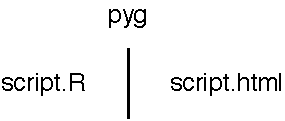
\includegraphics{../r-highlight.pdf}

Or a filter may take source code and transform it by running it through an interpreter and returning the transcript:


\includegraphics{../r-transcript.pdf}

\vspace{0.5cm}

Here is an R script:
\tiny
\begin{Verbatim}
<< d['hello.R'] >>
\end{Verbatim}
\small

And here is this same R script after passing through the 'r' filter:

\tiny
\begin{Verbatim}
<< d['hello.R|r'] >>
\end{Verbatim}
\small

You can run text through multiple filters chained together, so that each filter runs on the output of the previous filter:

\vspace{0.5cm}

\includegraphics{../r-transcript-highlight.pdf}
\vspace{0.5cm}

Here is the output of the R script after passing through the 'r' filter and then the 'pyg' filter for (rather subtle in this case) syntax highlighting:
\tiny
<< d['hello.R|r|pyg|l'] >>
\small

It is significant that we start with a file called 'script.R'. In Dexy, you write your code in standalone files and use the filtering system to pull this code into your document after it has been transformed in some way (there is a dummy filter called 'dexy' which pulls in the original unmodified text if you don't want it transformed in any way). There are many advantages to this approach of having source code live in its own separate files, as opposed to the approach taken by tools such as noweb where you have code blocks typed in delimited sections within a document. You can re-use the same source code in several places within a single document, and in various different formats within a single document, all of which will be kept in sync (because they all come from the same source file). You can also re-use code examples in multiple different documents. You can run the file outside of Dexy too, since it's just a normal code file with the expected file extension. In fact, you can use Dexy to document files in situ, especially with Dexy's remote URL feature which lets you fetch remote files, say from a version control system, and transform them with filters. And because you are working with normal code files you can continue to use your favourite text editor or IDE without having to change modes for Dexy.

\subsubsection*{Filter Examples}

Filters are responsible for most of Dexy's functionality, they are also the main way in which you can customize Dexy, and they have been designed to be easy to write. For example, here is a filter which just returns the first ten lines of the text it is passed:

\tiny
<< d['classes.json']['dexy.filters.python_filters.HeadFilter']['source'] >>
\small

That's the whole thing! For simple filters like this one, you only need to define a process\_text method which returns the transformed text. The ALIASES constant defines how you can refer to this filter to tell Dexy that you want to apply it. So for this filter, you would write ``$long.txt|head$'' to indicate that you wanted to invoke the 'head' filter on the contents of the file long.txt.

As mentioned earlier, splitting documents into sections is an important capability of Dexy since it allows you to write, say, tutorials with the code sample presented in bite-size chunks which can be easily and clearly explained. This sectioning is implemented by the Idiopidae filter, which implements a process\_text\_to\_dict() method:
\tiny
<< d['classes.json']['dexy.filters.pygments_filters.PygmentsFilter']['source'] >>
\small

If you wish to split your file up into sections using some other system then you just need to implement a similar filter which implements process\_text\_to\_dict().

Some filters take care to preserve this sectioning. For example here is a Python filter which runs each section of code through the Python interpreter, while preserving the names of each section. Importantly this all happens within a single Python session so that variable names etc. are preserved between sections.

\tiny
<< d['classes.json']['dexy.filters.process_filters.SubprocessFilter']['source'] >>
\small

The process\_dict() method expects you to accept a dict and return another dict.

The DexyHandler class defines a default process() method which looks to see if you have defined a process\_text(), process\_dict(), or process\_text\_to\_dict() method in your subclass:

\tiny
<< d['source.json']['dexy.dexy_filter.DexyFilter.process'] >>
\small

If you define more than one of these, Dexy raises an error. Dexy also raises an error if you try to pipe content which is in sections through a process\_text() method as this won't preserve the sections.

So, you can create a filter by subclassing DexyHandler and implementing one of the three special method names, or if you need more control you can override the process() method itself, as in the dot handler:

\tiny
<< d['classes.json']['dexy.filters.subprocess_filters.DotFilter']['source'] >>
\small

\vspace{1cm}

The dot handler takes dot code like this:
\tiny
\begin{Verbatim}
<< d['example.dot'] >>
\end{Verbatim}
\small

And renders it using graphviz:

\includegraphics{<< a['example.dot|dot|p'].filename() >>}

The 'latex' filter which was used to render this newspaper into PDF is another example of a filter which overrides the process() method:

\tiny
<< d['classes.json']['dexy.filters.subprocess_filters.LatexFilter']['source'] >>
\small

\subsubsection*{Templating}

The most important filter right now is probably the Jinja filter. Jinja is a templating system which allows you to place special tags in your document to indicate that dynamic content should go there. This is how you can write a document and pull in the output of running your source code files through various filters. Because the support for Jinja has been implemented as a filter, Dexy will be able to support other templating systems very easily (Python-based systems most easily), although for now Jinja is the only supported system.

Much of the work of the Jinja filter is in making available the output of the various filters that have been run. Actually running Jinja itself is only a few lines of code. The documentation at http://jinja.pocoo.org is the best source of reference for what you can do with Jinja, bearing in mind that for \LaTeX~documents Dexy automatically changes the jinja tag style from curly brackets to angle brackets so as to avoid clashing with \LaTeX's use of curly brackets.

Here is the source of the Jinja handler:

\tiny
<< d['classes.json']['dexy.filters.templating_filters.JinjaTextFilter']['source'] >>
\small

\subsubsection*{Dependencies, Topological Sort and Smart Caching}

What makes Dexy interesting and useful is that a document A (such as $article.html|jinja$) can depend on another document B (such as $script.R|pyg$). So, we need a way to tell Dexy that A depends on B. Then Dexy needs to figure out that B needs to be processed first, and Dexy needs to have a way of making the output of B available to A.

We tell Dexy which items to process and what the dependencies are using a specification file. Then Dexy implements a topological sort to determine an order for the documents so that all dependencies are processed first. Dexy then processes the documents in order, and stores the output in a special directory using carefully chosen filenames. The filenames are chosen so that if you run Dexy again and nothing has changed in the source, Dexy will use its stored version of the file rather than running the filters gain. This saves a lot of time, especially if you have a large document which depends on dozens of other files and only 1 of them has changed.

Here is the specification file for this newspaper.

\tiny
\begin{Verbatim}
<< d['.dexy'] >>
\end{Verbatim}
\small

This is a rather complex specification, but you can see that some files are listed by name with specific other files mentioned as inputs. Other directives are wildcard directives which apply to all files with a given extension. Names starting with @ are `virtual' files, there isn't a file called artifact.py in this directory, but Dexy will fetch the contents at the specified URL and pretend this is a local file called artifact.py, which is then put through the 'pyg' filter for syntax highlighting. The 'l' filter doesn't do anything itself, but it forces the output to have a .tex file extension, and this tells 'pyg' to use \LaTeX~formatting codes rather than the default of HTML. Many filters change their behaviour depending on the file extension accepted by the next filter in the chain.

Dexy's Controller class processes the config, builds up a list of all files needing to be processed and determines the ordering to use:

\tiny
<< d['source.json']['dexy.controller.Controller.process_config']['1'] >>
\small

This is the topological sort algorithm which is used:

\tiny
<< d['source.json']['dexy.topsort.topsort'] >>
\small

The Document class is responsible for actually processing the specified filters:

\tiny
<< d['source.json']['dexy.document.Document.run'] >>
\small

With the results of each step being cached by the Artifact class.

\tiny
<< d['source.json']['dexy.artifact.Artifact.setup'] >>
\small

The artifact object calculates a hashstring to identify its contents:

\tiny
<< d['source.json']['dexy.artifact.Artifact.set_hashstring'] >>
\small

And uses this hashstring for the stored filename:

\tiny
<< d['source.json']['dexy.artifact.Artifact.filename'] >>
\small

Thus we see the interaction of the specification, the topological sort, and Dexy's smart caching.

\subsubsection*{Dexy's Interface}

Dexy is run via a command line tool, a web-based interface to Dexy is also in development. Calling Dexy with the -h flag shows the available command line options:
\tiny
<< d['dexy.sh|pyg|l'] >>
\small

Currently these options are as follows:

\tiny
\begin{Verbatim}
<< d['dexy.sh|bash'] >>
\end{Verbatim}
\small

Dexy requires a number of directories to be present when it is run. This is because Dexy uses these directories, but also to make sure that you are in an appropriate location and are aware that Dexy will be generating lots of files in this location. You can call dexy with the --setup flag to create these directories for you, and you can also specify a different name to be used for any of these standard directories in case they should conflict with files already present in your system.

Dexy writes to a log file in logs/dexy.log and it is recommended that you tail -f this file while you are working. If you run into difficulties with your documents, then this log file is the first place you should look for clues. The log file also tells you where the results of processing files have been stored

\tiny
\begin{Verbatim}
newspaper.tex -> artifacts/d21c030ce79ea164c7cfe78549916dc9.tex
newspaper.tex|jinja -> artifacts/88088ef5e3fe631e7d44c7bcbe5f0b2e.tex
newspaper.tex|jinja|latex -> artifacts/df3a5eaafa2ded1723914268d5e6eafd.pdf
\end{Verbatim}
\small

The final steps are written to more canonical filenames in the cache/ directory, this is also indicated in the log

\tiny
\begin{Verbatim}
saving artifacts/df3a5eaafa2ded1723914268d5e6eafd.pdf to 
     cache/newspaper/newspaper.tex-jinja-latex.pdf
\end{Verbatim}
\small

If you want simpler canonical filenames, you can use the -s or --short flag in which case the output would simply be newspaper.pdf, i.e. the original file base name with the final file extension. The website at http://dexy.it is generated in this way.



\pagebreak

\subsection*{Source of this Newspaper}

This is the beginning of the .tex file containing the source for this newspaper. This shows you the LaTeX preamble and also some Jinja tags for including dynamic Dexy content. Full source code is available from http://bitbucket.org/ananelson/dexy-examples/newspaper

\tiny
<< d['newspaper.tex|wrap|pyg|l'] >>
\small


\includegraphics{../grid.pdf}

\end{multicols*}

\end{document}
